\documentclass[11pt,letterpaper]{article}

\usepackage[letterpaper,margin=0.75in,nohead]{geometry}

\usepackage{xcolor}

% add packages as needed
\usepackage{graphicx}
\usepackage{subcaption}
\usepackage[colorlinks]{hyperref}
\hypersetup{colorlinks,
citecolor=blue
}
\usepackage{url}
\usepackage{breakurl}

\title{CIS 6930: Privacy \& Machine Learning\\
	\Large Final Project Report: \textcolor{blue}{\bf Deep learning-based approach for stylometric De-Anonymization for model authorship}} %% TODO: replace with the title of your project

%% TODO: your name and email go here (all members of the group)
%% Comment out as needed and designate a point of contact
\author{
        Apoorv Chandurkar \\{\em (Point of Contact)} \\
        apoorvchandurkar@ufl.edu\\
        \and
        Kunwardeep Singh \\
        kunwardeep.singh@ufl.edu\\
}

% set the date to today
\date{\today}


\begin{document} % start document tag

\maketitle


%%% Remember: writing counts! (try to be clear and concise.)
%%% the final report should be 4+ page (in 11pt font)


%% TODO: you decide the structure!
%% Make sure the report:
%% - is self-contained; introduces background concepts & related work as needed
%% - contains results (even if preliminary)!!
%% - has an appropriate structure and is well written (e.g., proofread at least once!)
%%
%% Example structure:
%\section{Introduction}
%\section{Background \& Related Work}
%\section{Methodology}
%\section{Datasets}
%\section{Experimental Results}
%\section{Conclusions}

% TODO:
\section{Introduction}

With the rapid advancement in Natural Language Processing and 
Deep learning, the end-to-end pipeline for many natural 
language-related tasks is possible. New architectures for Language 
modeling are now achieving impressive results in Natural Language 
Generation which can output coherent text given some textual prompt. 
However, there is a concern that the misuse of these models can be 
done by spreading fake news and malicious content on a large scale. 
Hence, from a security perspective, it is imperative to treat these
models as potential authors and perform a stylometric analysis of 
the text they are generating to de-anonymize them to check if 
they are deployed with malicious intent. In this project, we 
have developed a Deep-learning based classifier that can classify 
text generated by the top 3 State of the Art open-source Language 
Models. Our goal is to research how much effect the architecture of 
a neural network has on its text generation style if any. We aim to 
find out if there is something unique about the text being generated 
by the model and if we can use this property to de-anonymize the text.
We add another class of human-generated text and examine how much 
stylometric difference is present between current SoTA Language 
Models and human-written text.

\section{Background}
A statistical language model is a probability distribution over 
sequences of words. In machine learning problems in the domain of 
natural language processing, words are embedded into vectors and given 
as an input to neural networks to perform different tasks like classification, 
text summarization, question answering, text generation, etc. In the specific 
case of text generation, language modes are directly relevant to the final 
output of the neural model as text generated by sampling from the probability 
distribution of the language model which maximizes the overall probability of 
the sequence of tokens. \par 
Earlier research used recurrent neural networks and their derivatives 
like Gated Recurrent Unit or Long-Short Term Memory (LSTM) networks to 
model a probability distribution over a set of vocabulary. Then, 
Transformer\cite{vaswani2017attention} based architecture was introduced which used the concept 
of attention, which addressed the issue of sequential processing and 
limitation of long-term dependency tracking. Hence, there was a significant 
increase in the SoTA performance on various Natural Language Processing 
benchmarks. In February 2019, OpenAI released the GPT- 2\cite{radford2019language} model paper 
in which they said that only training a large network of 1.5 Billion 
parameters to predict the next word given a previous sequence was enough 
to achieve SoTA performance in text generation task. This was just a 
scaled-up version of the original transformer-based GPT\cite{radford2018improving} model. 
Also, XLNET\cite{yang2019xlnet} architecture released which is a large scale 
transformer-based architecture currently having a top - 5 leaderboard 
position for the general-purpose NLP task-based GLUE\cite{wang2018glue} benchmark.

\section{Related Work}
De-anonymization of anonymous authors through stylometry has been used 
historically to get literary, historical and criminal investigation 
breakthroughs. Stylometry was earlier done only manually to identify 
hidden attributes associated with authors helping in the de-anonymization 
process. With the advent of machine learning researchers in the security 
domain have applied machine learning to classify text or attribute 
authorship based on authorship style or genre. (for eg. Afroz et al. \cite{afroz2014doppelganger}, 
Ramyaa et al. \cite{ramyaa2004using}) But in these methods, the features based on which 
classification is done are hand-crafted and extracted manually. Also, 
Caliskan-Islam et al \cite{caliskan2015anonymizing} used stylometry on programming code to 
de-anonymize programmers who authored the source code using a Random 
Forest based classifier. Many papers use stylometry to only predict 
some personal attributes of the author like gender and/or age etc.(for 
eg. Sarawgi et al. \cite{sarawgi2011gender}, Surendran et al.\cite{surendran2017stylometry}). We are proposing to use 
Deep Learning to classify input text without any completely manual feature 
extraction method. Also, we are proposing a novel idea of treating 
AI-models as authors and differentiating between their stylometric 
style along with researching style differences between humans and 
Language models.

\section{Data Generation}
We picked the top 3 State of The Art language models in the 
literature, namely, OpenAI GPT, GPT2 and XL-NET. After looking and 
testing different open-source implementation of these models, we 
decided to use the HuggingFace transformer library 
(https://github.com/huggingface/transformers) \cite{Wolf2019HuggingFacesTS} for selecting and 
generating text. We studied the Transformers library, which has the 
option to choose and fine-tune many hyperparameters at the text 
generation phase. We decided on many hyperparameters like no. of tokens 
generated by the model and input prompt given to the text. \par
We discussed that to be consistent across different models, input 
prompt given to generate text should be the same for all models. 
This will help in defining the classification task as each model 
will produce text based on the same context in the same domain. 
Hence, our de-anonymization classifier will be incentivized to 
discriminate based on the content structure rather than only looking 
at the individual tokens of the text. \par
After surveying many NLP based text datasets, we decided to use the 
OpinRank review dataset (https://github.com/kavgan/OpinRank) \cite{ganesan2012opinion}, which is 
a dataset of cars and hotels reviews by customers. We focus on hotel 
reviews for our task. Our motivation for working with the reviews, 
in general, is that potential misuse of large scale text-generation 
models can be to generate fake positive or negative reviews to 
manipulate ratings and consumer sentiment on social media. \par
We generated 2000 reviews from each language model to create a total 
dataset of 6000 reviews. These models were given an input prompt of 
300 tokens initially and 100 token long reviews were generated as we 
found that 100 was the average word length for reviews in the dataset. \par


\clearpage

\section{Classification Problem}
We map the problem of “de-anonymization” into a classification task, 
where our multi-class classifier will categorize the input text to be 
between one of the categories it was trained on. \par
For such a “multi-token sequence to a categorical mapping”, we use 
LSTM neural network which is used primarily for such tasks. The final 
output layer will be changed according to the total number of classes 
in the classification task. The model architecture used is shown below:

\begin{verbatim}
_________________________________________________________________
Layer (type)                 Output Shape              Param #   
=================================================================
embedding_1 (Embedding)      (None, 100, 100)          5000000   
_________________________________________________________________
spatial_dropout1d_1 (Spatial (None, 100, 100)          0         
_________________________________________________________________
lstm_1 (LSTM)                (None, 100)               80400     
_________________________________________________________________
dense_1 (Dense)              (None, 4)                 404       
=================================================================
Total params: 5,080,804
Trainable params: 5,080,804
Non-trainable params: 0
_________________________________________________________________
\end{verbatim}

\section{Experimental Results}
To investigate the accuracy of the classifier in all the possible 
contexts, we compared each language model against each other along with 
classifying them against human-generated reviews as well. Finally, 
we train a multi-class classifier which classifies against all the 
models along with the human text. These are the results:
\begin{enumerate}
        \item GPT vs GPT-2 classifier results are shown in Fig \ref{fig:prob6.1}
        \item GPT vs XLNet classifier results are shown in Fig \ref{fig:prob6.2}
        \item GPT-2 vs XLNet classifier results are shown in Fig \ref{fig:prob6.3}
        \item GPT vs GPT-2 vs XLNet vs Human-written classifier results are shown in Fig \ref{fig:prob6.4}
\end{enumerate}

\begin{figure}[h!]
        \centering
        \begin{subfigure}[b]{1.0\linewidth}
                \centering
                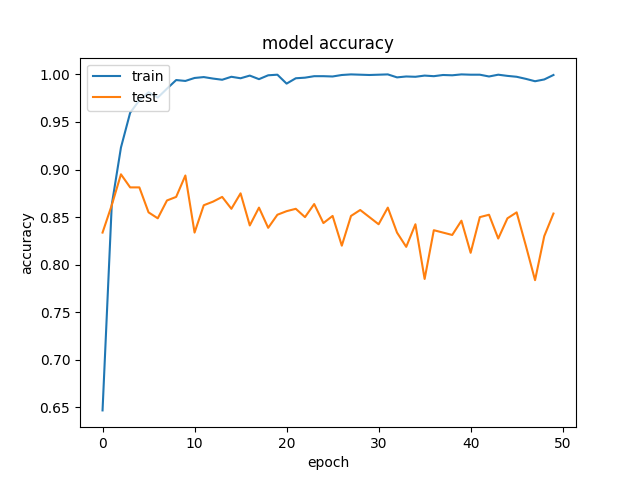
\includegraphics[width=0.7\linewidth]{accuracy_epochs_gpt1_gpt2.png}
                \caption{Accuracy}
        \end{subfigure}
        \begin{subfigure}[b]{1.0\linewidth}
                \centering
                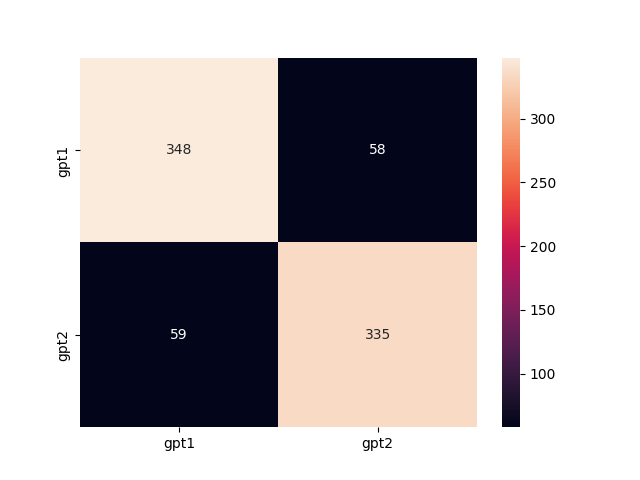
\includegraphics[width=0.7\linewidth]{sns_heatmap_gpt1_gpt2.png}
                \caption{Confusion Matrix}
        \end{subfigure}
        \caption{Classifier Performance GPT vs GPT-2. Validation accuracy is 85.12\%}
        \label{fig:prob6.1}
\end{figure}

\begin{figure}[h!]
        \centering
        \begin{subfigure}[b]{1.0\linewidth}
                \centering
                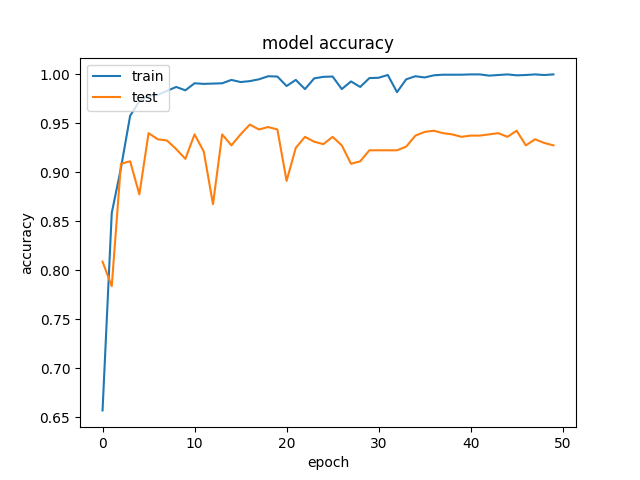
\includegraphics[width=0.7\linewidth]{accuracy_epochs_gpt1_xlnet.png}
                \caption{Accuracy}
        \end{subfigure}
        \begin{subfigure}[b]{1.0\linewidth}
                \centering
                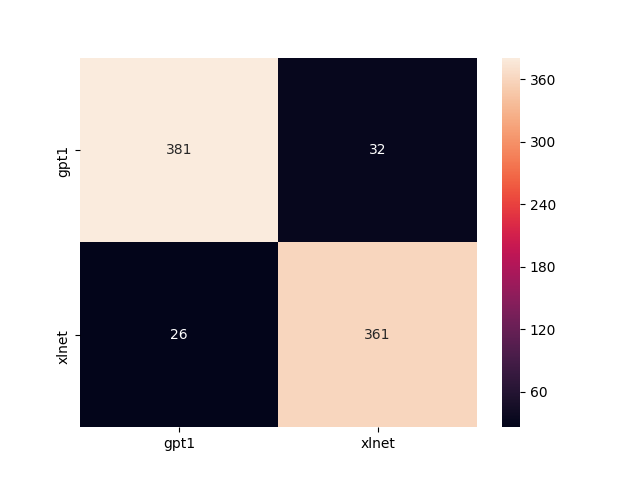
\includegraphics[width=0.7\linewidth]{sns_heatmap_gpt1_xlnet.png}
                \caption{Confusion Matrix}
        \end{subfigure}
        \caption{Classifier Performance GPT vs xlnet. Validation accuracy is 92.75\%}
        \label{fig:prob6.2}
\end{figure}

\begin{figure}[h!]
        \centering
        \begin{subfigure}[b]{1.0\linewidth}
                \centering
                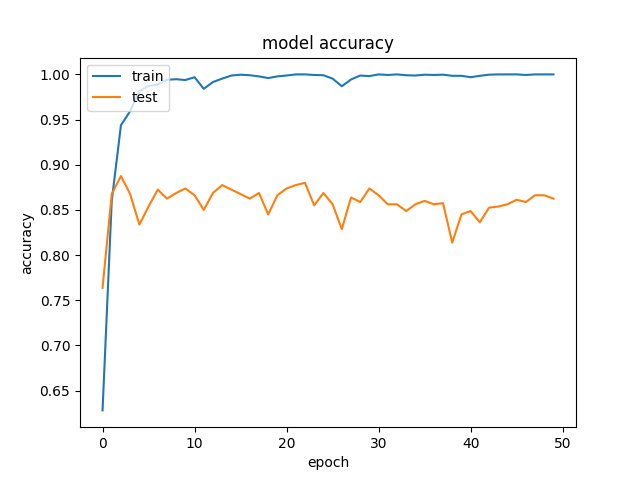
\includegraphics[width=0.7\linewidth]{accuracy_epochs_gpt2_xlnet.png}
                \caption{Accuracy}
        \end{subfigure}
        \begin{subfigure}[b]{1.0\linewidth}
                \centering
                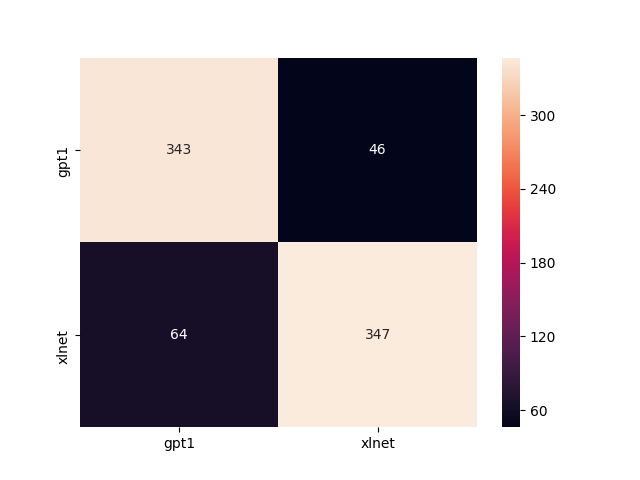
\includegraphics[width=0.7\linewidth]{sns_heatmap_gpt2_xlnet.png}
                \caption{Confusion Matrix}
        \end{subfigure}
        \caption{Classifier Performance GPT-2 vs xlnet. Validation accuracy is 86.25\%}
        \label{fig:prob6.3}
\end{figure}

\begin{figure}[h!]
        \centering
        \begin{subfigure}[b]{1.0\linewidth}
                \centering
                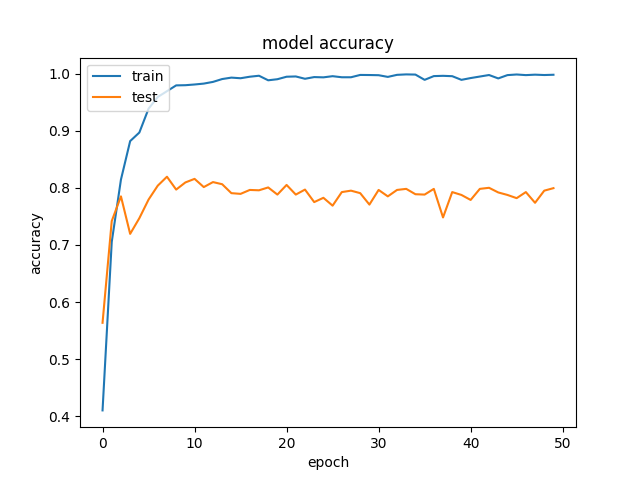
\includegraphics[width=0.7\linewidth]{accuracy_vs_epochs_all.png}
                \caption{Accuracy}
        \end{subfigure}
        \begin{subfigure}[b]{1.0\linewidth}
                \centering
                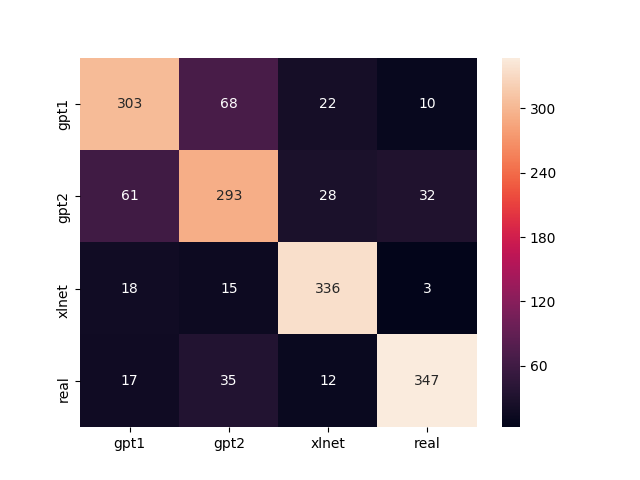
\includegraphics[width=0.7\linewidth]{sns_heatmap_all.png}
                \caption{Confusion Matrix}
        \end{subfigure}
        \caption{Classifier Performance GPT vs GPT-2 vs xlnet vs Human-written. Validation accuracy is 80\%}
        \label{fig:prob6.4}
\end{figure}

\section{Conclusion}
Following conclusions can be drawn from the results obtained:
\begin{enumerate}
        \item Classifier overfits to the training data achieving accuracy close to 99.5\% for almost all instances, but validation accuracy drops due to overfitting. We used dropout to add regularization but still, there seems to be a persistence of overfitting. We can explore other architectures of the classifier to alleviate this issue.
        \item Higher generalization can be achieved by adding more training data and training a larger model with added drop-out layers, we decided to keep the classifier architecture relatively small owing to larger training and generation times which hinder quick prototyping and hypothesis testing.
        \item In the case of 4 class classification, the classifier performed the worst between classifying GPT - 1 and GPT - 2,  which indicates the implicit text distribution is similar between models having the same architecture but different parameter scale.
        \item All of the accuracies are above the simple baseline of random chance, hence it can be said classifier is able to capture the difference but as the classifier mapping function from a sequence of tokens to a categorical value is highly non-linear, hence future research should be done on which will focus on the interpretability of the classification.
\end{enumerate}

\clearpage
\bibliographystyle{ieeetr}
\bibliography{References}

\end{document} % end tag of the document
